
\documentclass[a4paper,12pt]{article}
%%%%%%%%%%%%%%%%%%%%%%%%%%%%%%%%%%%%%%%%%%%%%%%%%%%%%%%%%%%%%%%%%%%%%%%%%%%%%%%%%%%%%%%%%%%%%%%%%%%%%%%%%%%%%%%%%%%%%%%%%%%%%%%%%%%%%%%%%%%%%%%%%%%%%%%%%%%%%%%%%%%%%%%%%%%%%%%%%%%%%%%%%%%%%%%%%%%%%%%%%%%%%%%%%%%%%%%%%%%%%%%%%%%%%%%%%%%%%%%%%%%%%%%%%%%%
\usepackage{eurosym}
\usepackage{vmargin}
\usepackage{amsmath}
\usepackage{graphics}
\usepackage{epsfig}
\usepackage{subfigure}
\usepackage{fancyhdr}
%\usepackage{listings}
\usepackage{framed}
\usepackage{graphicx}

\setcounter{MaxMatrixCols}{10}
%TCIDATA{OutputFilter=LATEX.DLL}
%TCIDATA{Version=5.00.0.2570}
%TCIDATA{<META NAME="SaveForMode" CONTENT="1">}
%TCIDATA{LastRevised=Wednesday, February 23, 2011 13:24:34}
%TCIDATA{<META NAME="GraphicsSave" CONTENT="32">}
%TCIDATA{Language=American English}

\pagestyle{fancy}
\setmarginsrb{20mm}{0mm}{20mm}{25mm}{12mm}{11mm}{0mm}{11mm}
\lhead{MA4128} \rhead{Mr. Kevin O'Brien}
\chead{Advanced Data Modelling}
%\input{tcilatex}


% http://www.norusis.com/pdf/SPC_v13.pdf
\begin{document}

\section{Dendrograms}
\begin{itemize}

\item A common way to visualize the cluster analysis’s progress is by drawing a
dendrogram, which displays the distance level at which there was a combination
of objects and clusters.
Here is an example of a dendrogram (which corresponds to the example in the next section of material.


%\begin{figure}[h!]
%	\begin{center}
%		% Requires \usepackage{graphicx}
%		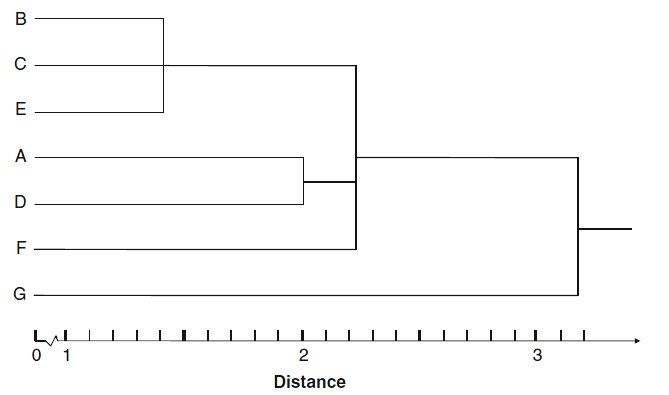
\includegraphics[scale=0.6]{images/Dendrogram.jpg}\\
%	\end{center}
%\end{figure}

\item An important question is how to decide on the number of
clusters to retain from the data. Unfortunately, hierarchical methods provide only
very limited guidance for making this decision. The only meaningful indicator
relates to the distances at which the objects are combined. Similar to factor
analysis’s scree plot, we can seek a solution in which an additional combination
of clusters or objects would occur at a greatly increased distance. This raises the
issue of what a great distance is, of course. For this purpose, we can make use of the dendrogram.

\item In constructing the dendrogram, SPSS rescales the distances to a range of 0–25; that is, the last merging step to a one-cluster solution takes place at a
(rescaled) distance of 25. The rescaling often lengthens the merging steps, thus
making breaks occurring at a greatly increased distance level more obvious. Despite this, this distance-based decision rule does not work very well in all
cases.

It is often difficult to identify where the break actually occurs. This is also
the case in our example above. By looking at the dendrogram, we could justify
a two-cluster solution ([A,B,C,D,E,F] and [G]), as well as a five-cluster solution
([B,C,E], [A], [D], [F], [G]).


\item 
The clustering algorithm is based on a distance measure that gives the best results if all variables are independent, continuous variables have a normal distribution (or categorical variables have a multinomial distribution). This is seldom the case in practice, but the algorithm is thought to behave reasonably well when the assumptions are not met.

\item 
Because cluster analysis does not involve hypothesis testing and calculation of observed significance levels, other than for descriptive follow-up, it's perfectly acceptable to cluster data that may not meet the assumptions for best performance.
\item 
The final outcome may depend on the order of the cases in the file. To minimize the effect, arrange the cases in random order. Sort them by the last digit of their ID numbers or something similar.
\end{itemize}
\end{document}